% Options for packages loaded elsewhere
\PassOptionsToPackage{unicode}{hyperref}
\PassOptionsToPackage{hyphens}{url}
\PassOptionsToPackage{dvipsnames,svgnames,x11names}{xcolor}
%
\documentclass[
  singlecolumn]{article}

\usepackage{amsmath,amssymb}
\usepackage{iftex}
\ifPDFTeX
  \usepackage[T1]{fontenc}
  \usepackage[utf8]{inputenc}
  \usepackage{textcomp} % provide euro and other symbols
\else % if luatex or xetex
  \usepackage{unicode-math}
  \defaultfontfeatures{Scale=MatchLowercase}
  \defaultfontfeatures[\rmfamily]{Ligatures=TeX,Scale=1}
\fi
\usepackage{lmodern}
\ifPDFTeX\else  
    % xetex/luatex font selection
\fi
% Use upquote if available, for straight quotes in verbatim environments
\IfFileExists{upquote.sty}{\usepackage{upquote}}{}
\IfFileExists{microtype.sty}{% use microtype if available
  \usepackage[]{microtype}
  \UseMicrotypeSet[protrusion]{basicmath} % disable protrusion for tt fonts
}{}
\makeatletter
\@ifundefined{KOMAClassName}{% if non-KOMA class
  \IfFileExists{parskip.sty}{%
    \usepackage{parskip}
  }{% else
    \setlength{\parindent}{0pt}
    \setlength{\parskip}{6pt plus 2pt minus 1pt}}
}{% if KOMA class
  \KOMAoptions{parskip=half}}
\makeatother
\usepackage{xcolor}
\usepackage[top=30mm,left=20mm,heightrounded]{geometry}
\setlength{\emergencystretch}{3em} % prevent overfull lines
\setcounter{secnumdepth}{-\maxdimen} % remove section numbering
% Make \paragraph and \subparagraph free-standing
\ifx\paragraph\undefined\else
  \let\oldparagraph\paragraph
  \renewcommand{\paragraph}[1]{\oldparagraph{#1}\mbox{}}
\fi
\ifx\subparagraph\undefined\else
  \let\oldsubparagraph\subparagraph
  \renewcommand{\subparagraph}[1]{\oldsubparagraph{#1}\mbox{}}
\fi

\usepackage{color}
\usepackage{fancyvrb}
\newcommand{\VerbBar}{|}
\newcommand{\VERB}{\Verb[commandchars=\\\{\}]}
\DefineVerbatimEnvironment{Highlighting}{Verbatim}{commandchars=\\\{\}}
% Add ',fontsize=\small' for more characters per line
\newenvironment{Shaded}{}{}
\newcommand{\AlertTok}[1]{\textcolor[rgb]{1.00,0.33,0.33}{\textbf{#1}}}
\newcommand{\AnnotationTok}[1]{\textcolor[rgb]{0.42,0.45,0.49}{#1}}
\newcommand{\AttributeTok}[1]{\textcolor[rgb]{0.84,0.23,0.29}{#1}}
\newcommand{\BaseNTok}[1]{\textcolor[rgb]{0.00,0.36,0.77}{#1}}
\newcommand{\BuiltInTok}[1]{\textcolor[rgb]{0.84,0.23,0.29}{#1}}
\newcommand{\CharTok}[1]{\textcolor[rgb]{0.01,0.18,0.38}{#1}}
\newcommand{\CommentTok}[1]{\textcolor[rgb]{0.42,0.45,0.49}{#1}}
\newcommand{\CommentVarTok}[1]{\textcolor[rgb]{0.42,0.45,0.49}{#1}}
\newcommand{\ConstantTok}[1]{\textcolor[rgb]{0.00,0.36,0.77}{#1}}
\newcommand{\ControlFlowTok}[1]{\textcolor[rgb]{0.84,0.23,0.29}{#1}}
\newcommand{\DataTypeTok}[1]{\textcolor[rgb]{0.84,0.23,0.29}{#1}}
\newcommand{\DecValTok}[1]{\textcolor[rgb]{0.00,0.36,0.77}{#1}}
\newcommand{\DocumentationTok}[1]{\textcolor[rgb]{0.42,0.45,0.49}{#1}}
\newcommand{\ErrorTok}[1]{\textcolor[rgb]{1.00,0.33,0.33}{\underline{#1}}}
\newcommand{\ExtensionTok}[1]{\textcolor[rgb]{0.84,0.23,0.29}{\textbf{#1}}}
\newcommand{\FloatTok}[1]{\textcolor[rgb]{0.00,0.36,0.77}{#1}}
\newcommand{\FunctionTok}[1]{\textcolor[rgb]{0.44,0.26,0.76}{#1}}
\newcommand{\ImportTok}[1]{\textcolor[rgb]{0.01,0.18,0.38}{#1}}
\newcommand{\InformationTok}[1]{\textcolor[rgb]{0.42,0.45,0.49}{#1}}
\newcommand{\KeywordTok}[1]{\textcolor[rgb]{0.84,0.23,0.29}{#1}}
\newcommand{\NormalTok}[1]{\textcolor[rgb]{0.14,0.16,0.18}{#1}}
\newcommand{\OperatorTok}[1]{\textcolor[rgb]{0.14,0.16,0.18}{#1}}
\newcommand{\OtherTok}[1]{\textcolor[rgb]{0.44,0.26,0.76}{#1}}
\newcommand{\PreprocessorTok}[1]{\textcolor[rgb]{0.84,0.23,0.29}{#1}}
\newcommand{\RegionMarkerTok}[1]{\textcolor[rgb]{0.42,0.45,0.49}{#1}}
\newcommand{\SpecialCharTok}[1]{\textcolor[rgb]{0.00,0.36,0.77}{#1}}
\newcommand{\SpecialStringTok}[1]{\textcolor[rgb]{0.01,0.18,0.38}{#1}}
\newcommand{\StringTok}[1]{\textcolor[rgb]{0.01,0.18,0.38}{#1}}
\newcommand{\VariableTok}[1]{\textcolor[rgb]{0.89,0.38,0.04}{#1}}
\newcommand{\VerbatimStringTok}[1]{\textcolor[rgb]{0.01,0.18,0.38}{#1}}
\newcommand{\WarningTok}[1]{\textcolor[rgb]{1.00,0.33,0.33}{#1}}

\providecommand{\tightlist}{%
  \setlength{\itemsep}{0pt}\setlength{\parskip}{0pt}}\usepackage{longtable,booktabs,array}
\usepackage{calc} % for calculating minipage widths
% Correct order of tables after \paragraph or \subparagraph
\usepackage{etoolbox}
\makeatletter
\patchcmd\longtable{\par}{\if@noskipsec\mbox{}\fi\par}{}{}
\makeatother
% Allow footnotes in longtable head/foot
\IfFileExists{footnotehyper.sty}{\usepackage{footnotehyper}}{\usepackage{footnote}}
\makesavenoteenv{longtable}
\usepackage{graphicx}
\makeatletter
\def\maxwidth{\ifdim\Gin@nat@width>\linewidth\linewidth\else\Gin@nat@width\fi}
\def\maxheight{\ifdim\Gin@nat@height>\textheight\textheight\else\Gin@nat@height\fi}
\makeatother
% Scale images if necessary, so that they will not overflow the page
% margins by default, and it is still possible to overwrite the defaults
% using explicit options in \includegraphics[width, height, ...]{}
\setkeys{Gin}{width=\maxwidth,height=\maxheight,keepaspectratio}
% Set default figure placement to htbp
\makeatletter
\def\fps@figure{htbp}
\makeatother

\input{/Users/joseph/GIT/latex/latex-for-quarto.tex}
\makeatletter
\@ifpackageloaded{tcolorbox}{}{\usepackage[skins,breakable]{tcolorbox}}
\@ifpackageloaded{fontawesome5}{}{\usepackage{fontawesome5}}
\definecolor{quarto-callout-color}{HTML}{909090}
\definecolor{quarto-callout-note-color}{HTML}{0758E5}
\definecolor{quarto-callout-important-color}{HTML}{CC1914}
\definecolor{quarto-callout-warning-color}{HTML}{EB9113}
\definecolor{quarto-callout-tip-color}{HTML}{00A047}
\definecolor{quarto-callout-caution-color}{HTML}{FC5300}
\definecolor{quarto-callout-color-frame}{HTML}{acacac}
\definecolor{quarto-callout-note-color-frame}{HTML}{4582ec}
\definecolor{quarto-callout-important-color-frame}{HTML}{d9534f}
\definecolor{quarto-callout-warning-color-frame}{HTML}{f0ad4e}
\definecolor{quarto-callout-tip-color-frame}{HTML}{02b875}
\definecolor{quarto-callout-caution-color-frame}{HTML}{fd7e14}
\makeatother
\makeatletter
\@ifpackageloaded{caption}{}{\usepackage{caption}}
\AtBeginDocument{%
\ifdefined\contentsname
  \renewcommand*\contentsname{Table of contents}
\else
  \newcommand\contentsname{Table of contents}
\fi
\ifdefined\listfigurename
  \renewcommand*\listfigurename{List of Figures}
\else
  \newcommand\listfigurename{List of Figures}
\fi
\ifdefined\listtablename
  \renewcommand*\listtablename{List of Tables}
\else
  \newcommand\listtablename{List of Tables}
\fi
\ifdefined\figurename
  \renewcommand*\figurename{Figure}
\else
  \newcommand\figurename{Figure}
\fi
\ifdefined\tablename
  \renewcommand*\tablename{Table}
\else
  \newcommand\tablename{Table}
\fi
}
\@ifpackageloaded{float}{}{\usepackage{float}}
\floatstyle{ruled}
\@ifundefined{c@chapter}{\newfloat{codelisting}{h}{lop}}{\newfloat{codelisting}{h}{lop}[chapter]}
\floatname{codelisting}{Listing}
\newcommand*\listoflistings{\listof{codelisting}{List of Listings}}
\usepackage{amsthm}
\theoremstyle{definition}
\newtheorem{definition}{Definition}[section]
\theoremstyle{remark}
\AtBeginDocument{\renewcommand*{\proofname}{Proof}}
\newtheorem*{remark}{Remark}
\newtheorem*{solution}{Solution}
\makeatother
\makeatletter
\makeatother
\makeatletter
\@ifpackageloaded{caption}{}{\usepackage{caption}}
\@ifpackageloaded{subcaption}{}{\usepackage{subcaption}}
\makeatother
\ifLuaTeX
  \usepackage{selnolig}  % disable illegal ligatures
\fi
\IfFileExists{bookmark.sty}{\usepackage{bookmark}}{\usepackage{hyperref}}
\IfFileExists{xurl.sty}{\usepackage{xurl}}{} % add URL line breaks if available
\urlstyle{same} % disable monospaced font for URLs
\hypersetup{
  pdftitle={Causal diagrams: Five elementary structures},
  pdfauthor={Joseph Bulbulia},
  colorlinks=true,
  linkcolor={blue},
  filecolor={Maroon},
  citecolor={Blue},
  urlcolor={Blue},
  pdfcreator={LaTeX via pandoc}}

\title{Causal diagrams: Five elementary structures}
\author{Joseph Bulbulia}
\date{2023-03-04}

\begin{document}
\maketitle

\renewcommand*\contentsname{Table of contents}
{
\hypersetup{linkcolor=}
\setcounter{tocdepth}{3}
\tableofcontents
}
\begin{tcolorbox}[enhanced jigsaw, colback=white, rightrule=.15mm, opacityback=0, toptitle=1mm, bottomtitle=1mm, toprule=.15mm, bottomrule=.15mm, colbacktitle=quarto-callout-note-color!10!white, left=2mm, titlerule=0mm, colframe=quarto-callout-note-color-frame, coltitle=black, title=\textcolor{quarto-callout-note-color}{\faInfo}\hspace{0.5em}{Readings}, arc=.35mm, leftrule=.75mm, breakable, opacitybacktitle=0.6]

\begin{itemize}
\tightlist
\item
  Barrett M (2023). \emph{ggdag: Analyze and Create Elegant Directed
  Acyclic Graphs}. R package version 0.2.7.9000,
  \url{https://github.com/malcolmbarrett/ggdag}
\item
  ``An Introduction to Directed Acyclic Graphs'',
  \url{https://r-causal.github.io/ggdag/articles/intro-to-dags.html}
\item
  ``Common Structures of Bias'',
  \url{https://r-causal.github.io/ggdag/articles/bias-structures.html}
\end{itemize}

\end{tcolorbox}

\begin{tcolorbox}[enhanced jigsaw, colback=white, rightrule=.15mm, opacityback=0, toptitle=1mm, bottomtitle=1mm, toprule=.15mm, bottomrule=.15mm, colbacktitle=quarto-callout-important-color!10!white, left=2mm, titlerule=0mm, colframe=quarto-callout-important-color-frame, coltitle=black, title=\textcolor{quarto-callout-important-color}{\faExclamation}\hspace{0.5em}{Key concepts for the test(s):}, arc=.35mm, leftrule=.75mm, breakable, opacitybacktitle=0.6]

\begin{itemize}
\tightlist
\item
  \textbf{Confounding} (introduced in week 2)
\item
  \textbf{Internal Validity} (introduced in week 2)
\item
  \textbf{External Validity} (introduced in week 3)
\end{itemize}

\end{tcolorbox}

\begin{tcolorbox}[enhanced jigsaw, colback=white, rightrule=.15mm, opacityback=0, toptitle=1mm, bottomtitle=1mm, toprule=.15mm, bottomrule=.15mm, colbacktitle=quarto-callout-important-color!10!white, left=2mm, titlerule=0mm, colframe=quarto-callout-important-color-frame, coltitle=black, title=\textcolor{quarto-callout-important-color}{\faExclamation}\hspace{0.5em}{Download Your Laboratory R Script Here}, arc=.35mm, leftrule=.75mm, breakable, opacitybacktitle=0.6]

Assuming you have installed R and RStudio:

\begin{enumerate}
\def\labelenumi{\arabic{enumi}.}
\item
  Download the R script for Lab 01 by clicking the link below. This
  script contains the code you will work with during your laboratory
  session.
\item
  After downloading, open RStudio.
\item
  In RStudio, create a new R script file by going to
  \texttt{File\ \textgreater{}\ New\ File\ \textgreater{}\ R\ Script}.
\item
  Copy the contents of the downloaded \texttt{.R} file and paste them
  into the new R script file you created in RStudio.
\item
  Save the new R script file in your project directory for easy access
  during the lab.
\end{enumerate}

\href{https://raw.githubusercontent.com/go-bayes/psyc-434-2024/main/laboratory/01-lab.R}{Download
the R script for Lab 01}

\end{tcolorbox}

\subsection{Overview}\label{overview}

\begin{itemize}
\tightlist
\item
  Understanding causal diagrams: definitions and applications
\item
  Introduction to five elementary structures and four rules in causal
  inference
\item
  Introduction to R interface and data simulation
\end{itemize}

\subsection{Review}\label{review}

\begin{enumerate}
\def\labelenumi{\arabic{enumi}.}
\item
  All research begins with a question. Our question should be stated
  first. What do we want to know? For whom does this knowledge apply?
\item
  In psychological research, we typically want to understand the causes
  and consequences of thought and behaviour - ``What if?'' questions.
\item
  The following concepts help us to describe two types of failure mode:
\end{enumerate}

\begin{itemize}
\item
  \textbf{External Validity}: the extent to which the findings of a
  study can be generalised to other situations, people, settings, and
  time periods. That is, we want to know if our findings carry beyond
  the \emph{sample population} to the \emph{target population}. We fail
  when our study does not generalise as we think.
\item
  \textbf{Internal Validity}: the degree to which a study can
  demonstrate that a causal relationship exists between the
  `independent' and `dependent' variables, free of confounding. In this
  course, we will use the terms ``outcome'' and ``treatment'' in place
  of ``independent'' and ``dependent''.\footnote{We use the terms
    ``treatment'' and ``outcome'' because ``What if?'' questions
    implicitly invoke the idea of intervening on the world. ``If we did
    this, \emph{then} what would happen to that\ldots?}
\end{itemize}

\begin{enumerate}
\def\labelenumi{\arabic{enumi}.}
\setcounter{enumi}{4}
\tightlist
\item
  Our focus in the first four weeks of the course: challenges to
  internal validity from \textbf{confounding bias.}
\end{enumerate}

\begin{definition}[]\protect\hypertarget{def-confounding}{}\label{def-confounding}

We say there is

\end{definition}

\subsection{Download Your Laboratory R Script
Here}\label{download-your-laboratory-r-script-here-1}

Assuming you have installed R and RStudio:

\begin{enumerate}
\def\labelenumi{\arabic{enumi}.}
\item
  Download the R script for Lab 01 by clicking the link below. This
  script contains the code you will work with during your laboratory
  session.
\item
  After downloading, open RStudio.
\item
  In RStudio, create a new R script file by going to
  \texttt{File\ \textgreater{}\ New\ File\ \textgreater{}\ R\ Script}.
\item
  Copy the contents of the downloaded \texttt{.R} file and paste them
  into the new R script file you created in RStudio.
\item
  Save the new R script file in your project directory for easy access
  during the lab.
\end{enumerate}

\href{https://raw.githubusercontent.com/go-bayes/psyc-434-2024/main/laboratory/01-lab.R}{Download
the R script for Lab 01}

\subsection{Causal Diagrams -- or ``Causal Directed Acyclic
Graphs''}\label{causal-diagrams-or-causal-directed-acyclic-graphs}

\subsection{Lab -- Regression in R}\label{lab-regression-in-r}

\subsection{\texorpdfstring{Simulating Data in R:
\texttt{Outcome\ \textasciitilde{}\ Treatment}}{Simulating Data in R: Outcome \textasciitilde{} Treatment}}\label{simulating-data-in-r-outcome-treatment}

\paragraph{Step 1: Set Up Your R
Environment}\label{step-1-set-up-your-r-environment}

Ensure R or RStudio is installed and open.

\paragraph{Step 2: Set a Seed for
Reproducibility}\label{step-2-set-a-seed-for-reproducibility}

To ensure that your simulated data can be reproduced exactly, it's good
practice to set a seed before generating random data. This makes your
analyses and simulations replicable.

\begin{Shaded}
\begin{Highlighting}[]
\FunctionTok{set.seed}\NormalTok{(}\DecValTok{123}\NormalTok{) }\CommentTok{\# use any number to set the seed}
\end{Highlighting}
\end{Shaded}

\paragraph{Step 3: Simulating Continuous
Data}\label{step-3-simulating-continuous-data}

To simulate continuous data, you can use functions like \texttt{rnorm()}
for normal distributions, \texttt{runif()} for uniform distributions,
etc. Here we simulate 100 normally distributed data points with a mean
of 50 and a standard deviation of 10:

\begin{Shaded}
\begin{Highlighting}[]
\NormalTok{n }\OtherTok{\textless{}{-}} \DecValTok{100} \CommentTok{\# number of observations}
\NormalTok{mean }\OtherTok{\textless{}{-}} \DecValTok{50}
\NormalTok{sd }\OtherTok{\textless{}{-}} \DecValTok{10}
\NormalTok{data\_continuous }\OtherTok{\textless{}{-}} \FunctionTok{rnorm}\NormalTok{(n, mean, sd)}

\CommentTok{\# view}
\FunctionTok{head}\NormalTok{(data\_continuous)}
\end{Highlighting}
\end{Shaded}

\begin{verbatim}
[1] 44.39524 47.69823 65.58708 50.70508 51.29288 67.15065
\end{verbatim}

\paragraph{Step 4: Simulating Categorical
Data}\label{step-4-simulating-categorical-data}

Categorical data can be simulated using the \texttt{sample()} function.
Here, we simulate a binary variable (gender) with two levels for 100
observations. There is equal probability of assignment.

\begin{Shaded}
\begin{Highlighting}[]
\NormalTok{levels }\OtherTok{\textless{}{-}} \FunctionTok{c}\NormalTok{(}\StringTok{"Male"}\NormalTok{, }\StringTok{"Female"}\NormalTok{)}
\NormalTok{data\_categorical }\OtherTok{\textless{}{-}} \FunctionTok{sample}\NormalTok{(levels, n, }\AttributeTok{replace =} \ConstantTok{TRUE}\NormalTok{)}

\CommentTok{\# view}
\FunctionTok{head}\NormalTok{(data\_categorical)}
\end{Highlighting}
\end{Shaded}

\begin{verbatim}
[1] "Female" "Female" "Female" "Male"   "Female" "Female"
\end{verbatim}

To generate categories with unequal probabilities, you can use the
\texttt{sample()} function by specifying the \texttt{prob} parameter,
which defines the probability of selecting each level. This allows for
simulating categorical data where the distribution between categories is
not uniform.

Below is an example that modifies your initial code to create a
categorical variable with unequal probabilities for ``Male'' and
``Female''. Here is an example with unequal probabilities:

\begin{Shaded}
\begin{Highlighting}[]
\CommentTok{\# Define levels and number of observations}
\NormalTok{levels }\OtherTok{\textless{}{-}} \FunctionTok{c}\NormalTok{(}\StringTok{"Male"}\NormalTok{, }\StringTok{"Female"}\NormalTok{)}
\NormalTok{n }\OtherTok{\textless{}{-}} \DecValTok{100} \CommentTok{\# total number of observations}

\CommentTok{\# Generate categorical data with unequal probabilities}
\NormalTok{data\_categorical\_unequal }\OtherTok{\textless{}{-}} \FunctionTok{sample}\NormalTok{(levels, n, }\AttributeTok{replace =} \ConstantTok{TRUE}\NormalTok{, }\AttributeTok{prob =} \FunctionTok{c}\NormalTok{(}\FloatTok{0.3}\NormalTok{, }\FloatTok{0.7}\NormalTok{))}

\CommentTok{\# View the first few elements}
\FunctionTok{head}\NormalTok{(data\_categorical\_unequal)}
\end{Highlighting}
\end{Shaded}

In this example, the \texttt{prob} parameter is set to
\texttt{c(0.3,\ 0.7)}, indicating a 30\% probability for ``Male'' and a
70\% probability for ``Female''. This results in a simulated dataset
where approximately 30\% of the observations are ``Male'' and 70\% are
``Female'', reflecting the specified unequal probabilities. Adjust the
probabilities as needed to fit the scenario you wish to simulate.

\begin{Shaded}
\begin{Highlighting}[]
\FunctionTok{set.seed}\NormalTok{(}\DecValTok{123}\NormalTok{) }\CommentTok{\#  reproducibility}
\NormalTok{groupA\_scores }\OtherTok{\textless{}{-}} \FunctionTok{rnorm}\NormalTok{(}\DecValTok{100}\NormalTok{, }\AttributeTok{mean =} \DecValTok{100}\NormalTok{, }\AttributeTok{sd =} \DecValTok{15}\NormalTok{) }\CommentTok{\# simulate scores for group A}
\NormalTok{groupB\_scores }\OtherTok{\textless{}{-}} \FunctionTok{rnorm}\NormalTok{(}\DecValTok{100}\NormalTok{, }\AttributeTok{mean =} \DecValTok{105}\NormalTok{, }\AttributeTok{sd =} \DecValTok{15}\NormalTok{) }\CommentTok{\# simulate scores for group B}

\CommentTok{\# ombine into a data frame}
\NormalTok{scores\_df }\OtherTok{\textless{}{-}} \FunctionTok{data.frame}\NormalTok{(}\AttributeTok{Group =} \FunctionTok{rep}\NormalTok{(}\FunctionTok{c}\NormalTok{(}\StringTok{"A"}\NormalTok{, }\StringTok{"B"}\NormalTok{), }\AttributeTok{each =} \DecValTok{100}\NormalTok{), }\AttributeTok{Scores =} \FunctionTok{c}\NormalTok{(groupA\_scores, groupB\_scores))}

\CommentTok{\# commands to view data}
\FunctionTok{str}\NormalTok{(scores\_df)}
\end{Highlighting}
\end{Shaded}

\begin{verbatim}
'data.frame':   200 obs. of  2 variables:
 $ Group : chr  "A" "A" "A" "A" ...
 $ Scores: num  91.6 96.5 123.4 101.1 101.9 ...
\end{verbatim}

\begin{Shaded}
\begin{Highlighting}[]
\CommentTok{\# summary of columns}
\FunctionTok{summary}\NormalTok{(scores\_df)}
\end{Highlighting}
\end{Shaded}

\begin{verbatim}
    Group               Scores      
 Length:200         Min.   : 65.36  
 Class :character   1st Qu.: 92.59  
 Mode  :character   Median :101.38  
                    Mean   :102.37  
                    3rd Qu.:111.59  
                    Max.   :153.62  
\end{verbatim}

\begin{Shaded}
\begin{Highlighting}[]
\CommentTok{\# top rows}
\FunctionTok{head}\NormalTok{(scores\_df)}
\end{Highlighting}
\end{Shaded}

\begin{verbatim}
  Group    Scores
1     A  91.59287
2     A  96.54734
3     A 123.38062
4     A 101.05763
5     A 101.93932
6     A 125.72597
\end{verbatim}

\begin{Shaded}
\begin{Highlighting}[]
\CommentTok{\# bottom rows}
\FunctionTok{tail}\NormalTok{(scores\_df)}
\end{Highlighting}
\end{Shaded}

\begin{verbatim}
    Group    Scores
195     B  85.33798
196     B 134.95820
197     B 114.01063
198     B  86.23093
199     B  95.83251
200     B  87.21780
\end{verbatim}

\subsection{Visualising simulated
data}\label{visualising-simulated-data}

Understanding your data visually is as important as the statistical
analysis itself. Let's create a simple plot to compare the score
distributions between the two groups.

\begin{Shaded}
\begin{Highlighting}[]
\ControlFlowTok{if}\NormalTok{ (}\SpecialCharTok{!}\FunctionTok{require}\NormalTok{(ggplot2)) \{}
  \FunctionTok{install.packages}\NormalTok{(}\StringTok{"ggplot2"}\NormalTok{)}
  \FunctionTok{library}\NormalTok{(ggplot2)}
\NormalTok{\} }\ControlFlowTok{else}\NormalTok{ \{}
  \FunctionTok{library}\NormalTok{(ggplot2)}
\NormalTok{\}}

\CommentTok{\# plot your data}
\FunctionTok{ggplot}\NormalTok{(scores\_df, }\FunctionTok{aes}\NormalTok{(}\AttributeTok{x =}\NormalTok{ Group, }\AttributeTok{y =}\NormalTok{ Scores, }\AttributeTok{fill =}\NormalTok{ Group)) }\SpecialCharTok{+}
  \FunctionTok{geom\_boxplot}\NormalTok{() }\SpecialCharTok{+}
  \FunctionTok{theme\_minimal}\NormalTok{() }\SpecialCharTok{+}
  \FunctionTok{labs}\NormalTok{(}\AttributeTok{title =} \StringTok{"Score Distribution by Group"}\NormalTok{, }\AttributeTok{x =} \StringTok{"Group"}\NormalTok{, }\AttributeTok{y =} \StringTok{"Scores"}\NormalTok{)}
\end{Highlighting}
\end{Shaded}

\begin{figure}[H]

{\centering 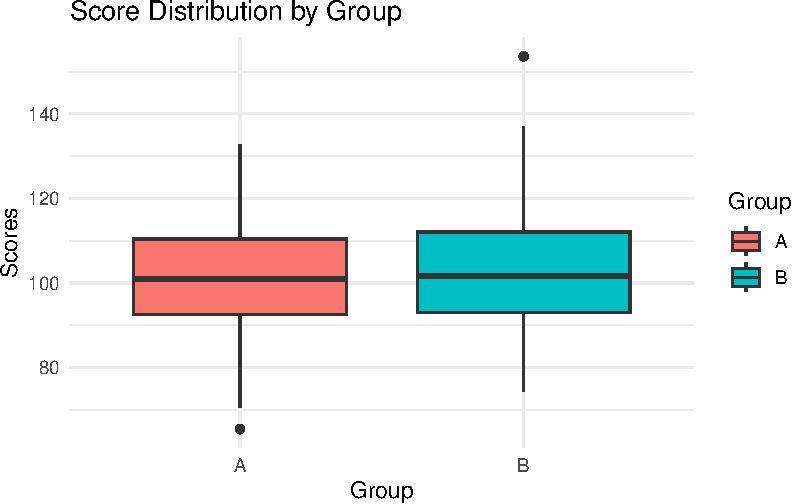
\includegraphics{02-content_files/figure-pdf/visualize-data-1.pdf}

}

\caption{Score Distribution by Group}

\end{figure}%

\subsection{Histogram}\label{sec-histogram}

\begin{Shaded}
\begin{Highlighting}[]
\FunctionTok{library}\NormalTok{(ggplot2)}

\CommentTok{\# H=histograms for both groups}
\FunctionTok{ggplot}\NormalTok{(scores\_df, }\FunctionTok{aes}\NormalTok{(}\AttributeTok{x =}\NormalTok{ Scores, }\AttributeTok{fill =}\NormalTok{ Group)) }\SpecialCharTok{+}
  \FunctionTok{geom\_histogram}\NormalTok{(}\AttributeTok{binwidth =} \DecValTok{5}\NormalTok{, }\AttributeTok{color =} \StringTok{"black"}\NormalTok{) }\SpecialCharTok{+}
  \FunctionTok{labs}\NormalTok{(}\AttributeTok{title =} \StringTok{"Distribution of Scores"}\NormalTok{,}
       \AttributeTok{x =} \StringTok{"Scores"}\NormalTok{,}
       \AttributeTok{y =} \StringTok{"Frequency"}\NormalTok{) }\SpecialCharTok{+}
  \FunctionTok{facet\_wrap}\NormalTok{(}\SpecialCharTok{\textasciitilde{}}\NormalTok{Group, }\AttributeTok{ncol =} \DecValTok{1}\NormalTok{)}
\end{Highlighting}
\end{Shaded}

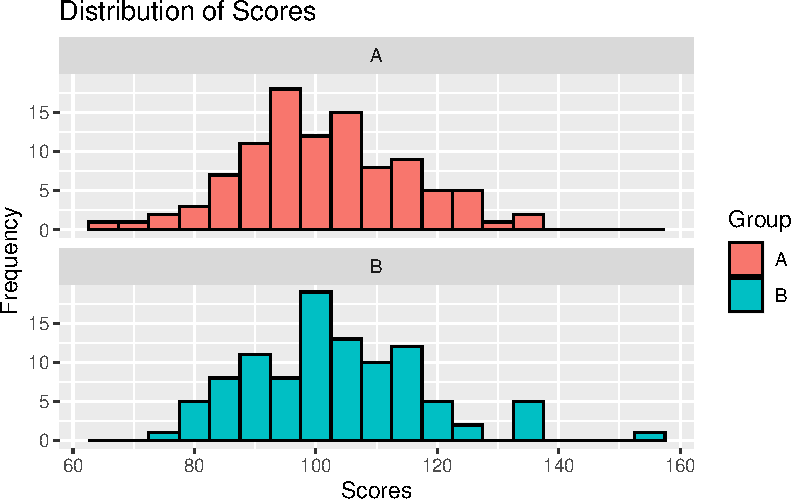
\includegraphics{02-content_files/figure-pdf/unnamed-chunk-6-1.pdf}

\subsection{Excercise 3}\label{excercise-3}

\begin{enumerate}
\def\labelenumi{\arabic{enumi}.}
\item
  Modify the simulation parameters to change each group's mean and
  standard deviation. Observe how these changes affect the distribution.
\item
  Go to the \hyperref[sec-histogram]{histogram}. Experiment with
  different bin widths. In your own words, how do large and small
  numbers speak differently to the data? When might you use one
  histogram and not another.
\end{enumerate}

\subsection{Simulating data for familiar statistical
tests}\label{simulating-data-for-familiar-statistical-tests}

\begin{Shaded}
\begin{Highlighting}[]
\CommentTok{\# simulate some data}
\NormalTok{data }\OtherTok{\textless{}{-}} \FunctionTok{rnorm}\NormalTok{(}\DecValTok{100}\NormalTok{, }\AttributeTok{mean =} \DecValTok{5}\NormalTok{, }\AttributeTok{sd =} \DecValTok{1}\NormalTok{) }\CommentTok{\# 100 random normal values with mean = 5}

\CommentTok{\# perform one{-}sample t{-}test}
\CommentTok{\# testing if the mean of the data is reliably different from 4}
\FunctionTok{t.test}\NormalTok{(data, }\AttributeTok{mu =} \DecValTok{4}\NormalTok{)}
\end{Highlighting}
\end{Shaded}

\begin{verbatim}

    One Sample t-test

data:  data
t = 11.796, df = 99, p-value < 2.2e-16
alternative hypothesis: true mean is not equal to 4
95 percent confidence interval:
 4.931989 5.308942
sample estimates:
mean of x 
 5.120465 
\end{verbatim}

\begin{Shaded}
\begin{Highlighting}[]
\CommentTok{\# simulate data for two groups}
\NormalTok{group1 }\OtherTok{\textless{}{-}} \FunctionTok{rnorm}\NormalTok{(}\DecValTok{50}\NormalTok{, }\AttributeTok{mean =} \DecValTok{5}\NormalTok{, }\AttributeTok{sd =} \DecValTok{1}\NormalTok{) }\CommentTok{\# 50 random normal values, mean = 5}
\NormalTok{group2 }\OtherTok{\textless{}{-}} \FunctionTok{rnorm}\NormalTok{(}\DecValTok{50}\NormalTok{, }\AttributeTok{mean =} \FloatTok{5.5}\NormalTok{, }\AttributeTok{sd =} \DecValTok{1}\NormalTok{) }\CommentTok{\# 50 random normal values, mean = 5.5}

\CommentTok{\# two{-}sample t{-}test}
\FunctionTok{t.test}\NormalTok{(group1, group2)}
\end{Highlighting}
\end{Shaded}

\begin{verbatim}

    Welch Two Sample t-test

data:  group1 and group2
t = -2.0293, df = 97.95, p-value = 0.04514
alternative hypothesis: true difference in means is not equal to 0
95 percent confidence interval:
 -0.837548023 -0.009343886
sample estimates:
mean of x mean of y 
 5.002054  5.425500 
\end{verbatim}

\begin{Shaded}
\begin{Highlighting}[]
\CommentTok{\# simulate pre{-}test and post{-}test scores}
\NormalTok{pre\_test }\OtherTok{\textless{}{-}} \FunctionTok{rnorm}\NormalTok{(}\DecValTok{30}\NormalTok{, }\AttributeTok{mean =} \DecValTok{80}\NormalTok{, }\AttributeTok{sd =} \DecValTok{10}\NormalTok{)}
\NormalTok{post\_test }\OtherTok{\textless{}{-}} \FunctionTok{rnorm}\NormalTok{(}\DecValTok{30}\NormalTok{, }\AttributeTok{mean =}\NormalTok{  pre\_test }\SpecialCharTok{+} \DecValTok{5}\NormalTok{, }\AttributeTok{sd =} \DecValTok{5}\NormalTok{) }\CommentTok{\# assume an increase}

\CommentTok{\# perform paired t{-}test}
\FunctionTok{t.test}\NormalTok{(pre\_test, post\_test, }\AttributeTok{paired =} \ConstantTok{TRUE}\NormalTok{)}
\end{Highlighting}
\end{Shaded}

\begin{verbatim}

    Paired t-test

data:  pre_test and post_test
t = -4.7761, df = 29, p-value = 4.725e-05
alternative hypothesis: true mean difference is not equal to 0
95 percent confidence interval:
 -6.785042 -2.716352
sample estimates:
mean difference 
      -4.750697 
\end{verbatim}

\subsubsection{\texorpdfstring{\textbf{Exercise 3: Linear Regression
Analysis with Simulated
Data}}{Exercise 3: Linear Regression Analysis with Simulated Data}}\label{exercise-3-linear-regression-analysis-with-simulated-data}

\paragraph{\texorpdfstring{\textbf{Task 1: Simulating Continuous
Treatment
Variable}}{Task 1: Simulating Continuous Treatment Variable}}\label{task-1-simulating-continuous-treatment-variable}

\begin{Shaded}
\begin{Highlighting}[]
\CommentTok{\# library for enhanced model reporting}
\FunctionTok{library}\NormalTok{(parameters)}

\CommentTok{\# set seed for reproducibility}
\FunctionTok{set.seed}\NormalTok{(}\DecValTok{123}\NormalTok{) }\CommentTok{\# choose a seed number for consistency}

\CommentTok{\# define the number of observations}
\NormalTok{n }\OtherTok{\textless{}{-}} \DecValTok{100} \CommentTok{\# total observations}

\CommentTok{\# simulate continuous treatment variable A}
\NormalTok{a }\OtherTok{\textless{}{-}} \FunctionTok{rnorm}\NormalTok{(n, }\AttributeTok{mean =} \DecValTok{50}\NormalTok{, }\AttributeTok{sd =} \DecValTok{10}\NormalTok{) }\CommentTok{\# mean = 50, sd = 10 for A}

\CommentTok{\# specify the effect size of A on Y}
\NormalTok{beta\_a }\OtherTok{\textless{}{-}} \DecValTok{2} \CommentTok{\# explicit effect size}

\CommentTok{\# simulate outcome variable Y including an error term}
\NormalTok{y }\OtherTok{\textless{}{-}} \DecValTok{5} \SpecialCharTok{+}\NormalTok{ beta\_a }\SpecialCharTok{*}\NormalTok{ a }\SpecialCharTok{+} \FunctionTok{rnorm}\NormalTok{(n, }\AttributeTok{mean =} \DecValTok{0}\NormalTok{, }\AttributeTok{sd =} \DecValTok{20}\NormalTok{) }\CommentTok{\# Y = intercept + beta\_a*A + error}

\CommentTok{\# create a dataframe}
\NormalTok{df }\OtherTok{\textless{}{-}} \FunctionTok{data.frame}\NormalTok{(}\AttributeTok{a =}\NormalTok{ a, }\AttributeTok{y =}\NormalTok{ y)}

\CommentTok{\# view the structure and first few rows of the dataframe}
\FunctionTok{str}\NormalTok{(df)}
\FunctionTok{head}\NormalTok{(df)}
\end{Highlighting}
\end{Shaded}

\paragraph{\texorpdfstring{\textbf{Task 2: Exploring the Simulated
Data}}{Task 2: Exploring the Simulated Data}}\label{task-2-exploring-the-simulated-data}

Before moving on to regression analysis, ensure students understand the
structure and distribution of the simulated data. Encourage them to use
\texttt{summary()}, \texttt{plot()}, and other exploratory data analysis
functions.

\paragraph{\texorpdfstring{\textbf{Task 3: Regression Analysis of
Continuous Treatment
Effect}}{Task 3: Regression Analysis of Continuous Treatment Effect}}\label{task-3-regression-analysis-of-continuous-treatment-effect}

\begin{Shaded}
\begin{Highlighting}[]
\CommentTok{\# perform linear regression of Y on A}
\NormalTok{fit }\OtherTok{\textless{}{-}} \FunctionTok{lm}\NormalTok{(y }\SpecialCharTok{\textasciitilde{}}\NormalTok{ a, }\AttributeTok{data =}\NormalTok{ df)}

\CommentTok{\# display the regression model summary}
\FunctionTok{summary}\NormalTok{(fit)}

\CommentTok{\# report the model in a reader{-}friendly format}
\NormalTok{report\_fit }\OtherTok{\textless{}{-}}\NormalTok{ report}\SpecialCharTok{::}\FunctionTok{report}\NormalTok{(fit)}
\FunctionTok{print}\NormalTok{(report\_fit)}

\CommentTok{\# optionally, visualize the relationship}
\FunctionTok{plot}\NormalTok{(df}\SpecialCharTok{$}\NormalTok{a, df}\SpecialCharTok{$}\NormalTok{y, }\AttributeTok{main =} \StringTok{"Scatterplot of Y vs. A"}\NormalTok{, }\AttributeTok{xlab =} \StringTok{"Treatment (A)"}\NormalTok{, }\AttributeTok{ylab =} \StringTok{"Outcome (Y)"}\NormalTok{)}
\FunctionTok{abline}\NormalTok{(fit, }\AttributeTok{col =} \StringTok{"red"}\NormalTok{)}
\end{Highlighting}
\end{Shaded}

\subsection{Equivalence of ANOVA and
Regression}\label{equivalence-of-anova-and-regression}

We will simulate data in R to show that a one-way ANOVA is a special
case of linear regression with categorical predictors. We will give some
reasons for preferring regression (in some settings).

\subsection{Method}\label{method}

First, we simulate a dataset with one categorical independent variable
with three levels (groups) and a continuous outcome (also called a
``dependant'') variable. This setup allows us to apply both ANOVA and
linear regression for comparison.

\begin{Shaded}
\begin{Highlighting}[]
\CommentTok{\# nice tables}
\ControlFlowTok{if}\NormalTok{ (}\SpecialCharTok{!}\FunctionTok{require}\NormalTok{(parameters)) \{}
  \FunctionTok{install.packages}\NormalTok{(}\StringTok{"parameters"}\NormalTok{)}
  \FunctionTok{library}\NormalTok{(parameters)}
\NormalTok{\} }\ControlFlowTok{else}\NormalTok{ \{}
  \FunctionTok{library}\NormalTok{(parameters)}
\NormalTok{\}}


\FunctionTok{set.seed}\NormalTok{(}\DecValTok{321}\NormalTok{) }\CommentTok{\# reproducibility}
\NormalTok{n }\OtherTok{\textless{}{-}} \DecValTok{90} \CommentTok{\# total number of observations}
\NormalTok{k }\OtherTok{\textless{}{-}} \DecValTok{3} \CommentTok{\# number of groups}

\CommentTok{\# simulate independent variable (grouping factor)}
\NormalTok{group }\OtherTok{\textless{}{-}} \FunctionTok{factor}\NormalTok{(}\FunctionTok{rep}\NormalTok{(}\DecValTok{1}\SpecialCharTok{:}\NormalTok{k, }\AttributeTok{each =}\NormalTok{ n}\SpecialCharTok{/}\NormalTok{k))}

\CommentTok{\# inspect}
\FunctionTok{str}\NormalTok{(group)}
\end{Highlighting}
\end{Shaded}

\begin{verbatim}
 Factor w/ 3 levels "1","2","3": 1 1 1 1 1 1 1 1 1 1 ...
\end{verbatim}

\begin{Shaded}
\begin{Highlighting}[]
\CommentTok{\# simulate outcome variable}
\NormalTok{means }\OtherTok{\textless{}{-}} \FunctionTok{c}\NormalTok{(}\DecValTok{100}\NormalTok{, }\DecValTok{100}\NormalTok{, }\DecValTok{220}\NormalTok{) }\CommentTok{\# Mean for each group}
\NormalTok{sd }\OtherTok{\textless{}{-}} \DecValTok{15} \CommentTok{\# Standard deviation (same for all groups)}

\CommentTok{\# generate random data}
\NormalTok{y }\OtherTok{\textless{}{-}} \FunctionTok{rnorm}\NormalTok{(n, }\AttributeTok{mean =} \FunctionTok{rep}\NormalTok{(means, }\AttributeTok{each =}\NormalTok{ n}\SpecialCharTok{/}\NormalTok{k), }\AttributeTok{sd =}\NormalTok{ sd)}


\CommentTok{\# make data frame}
\NormalTok{df\_1 }\OtherTok{\textless{}{-}} \FunctionTok{cbind.data.frame}\NormalTok{(y, group)}

\NormalTok{anova\_model }\OtherTok{\textless{}{-}} \FunctionTok{aov}\NormalTok{(y }\SpecialCharTok{\textasciitilde{}}\NormalTok{ group, }\AttributeTok{data =}\NormalTok{ df\_1)}
\CommentTok{\# summary(anova\_model)}
\NormalTok{table\_anova }\OtherTok{\textless{}{-}} \FunctionTok{model\_parameters}\NormalTok{(anova\_model)}

\CommentTok{\# report the model}
\NormalTok{report}\SpecialCharTok{::}\FunctionTok{report}\NormalTok{(anova\_model)}
\end{Highlighting}
\end{Shaded}

\begin{verbatim}
The ANOVA (formula: y ~ group) suggests that:

  - The main effect of group is statistically significant and large (F(2, 87) =
689.11, p < .001; Eta2 = 0.94, 95% CI [0.92, 1.00])

Effect sizes were labelled following Field's (2013) recommendations.
\end{verbatim}

Next, we analyse the same data using linear regression. In R, regression
models automatically convert categorical variables into dummy variables.

\begin{Shaded}
\begin{Highlighting}[]
\CommentTok{\# for tables (just installed)}
\FunctionTok{library}\NormalTok{(parameters)}

\CommentTok{\# regression model }
\NormalTok{fit }\OtherTok{\textless{}{-}} \FunctionTok{lm}\NormalTok{(y }\SpecialCharTok{\textasciitilde{}}\NormalTok{ group, }\AttributeTok{data =}\NormalTok{ df\_1)}

\CommentTok{\# uncomment if you want an ordinary summary}
\CommentTok{\# summary(regression\_model)}

\NormalTok{table\_fit }\OtherTok{\textless{}{-}}\NormalTok{ parameters}\SpecialCharTok{::}\FunctionTok{model\_parameters}\NormalTok{(fit)}

\CommentTok{\# print table}
\NormalTok{table\_fit}
\end{Highlighting}
\end{Shaded}

\begin{verbatim}
Parameter   | Coefficient |   SE |           95% CI | t(87) |      p
--------------------------------------------------------------------
(Intercept) |      101.22 | 2.60 | [ 96.06, 106.39] | 38.98 | < .001
group [2]   |       -0.80 | 3.67 | [ -8.10,   6.50] | -0.22 | 0.827 
group [3]   |      117.67 | 3.67 | [110.37, 124.97] | 32.04 | < .001
\end{verbatim}

\begin{Shaded}
\begin{Highlighting}[]
\FunctionTok{library}\NormalTok{(parameters)}
\FunctionTok{library}\NormalTok{(report)}

\CommentTok{\# report the model}
\NormalTok{report\_fit }\OtherTok{\textless{}{-}} \FunctionTok{report\_parameters}\NormalTok{(fit)}

\CommentTok{\#print}
\NormalTok{report\_fit}
\end{Highlighting}
\end{Shaded}

\begin{verbatim}
  - The intercept is statistically significant and positive (beta = 101.22, 95% CI [96.06, 106.39], t(87) = 38.98, p < .001; Std. beta = -0.68, 95% CI [-0.76, -0.59])
  - The effect of group [2] is statistically non-significant and negative (beta = -0.80, 95% CI [-8.10, 6.50], t(87) = -0.22, p = 0.827; Std. beta = -0.01, 95% CI [-0.14, 0.11])
  - The effect of group [3] is statistically significant and positive (beta = 117.67, 95% CI [110.37, 124.97], t(87) = 32.04, p < .001; Std. beta = 2.04, 95% CI [1.91, 2.17])
\end{verbatim}

\subsection{Upshot}\label{upshot}

ANOVA partitions variance into between-group and within-group
components, while regression models the mean of the dependent variable
as a linear function of the independent (including categorical)
variables. For many questions, ANOVA is appropriate, however, when we
are comparing groups, we often want a finer-grained interpretation.
Regression is built for obtaining this finer grain understanding. We
will return to regression over the next few weeks and use regression to
hone your skills in R. Later, Along the way, you'll learn more about
data visualisation, modelling, and reporting.

\begin{Shaded}
\begin{Highlighting}[]
\CommentTok{\# graph the output of the parameters table}
\CommentTok{\# visualisation}
\FunctionTok{plot}\NormalTok{(table\_fit)}
\end{Highlighting}
\end{Shaded}

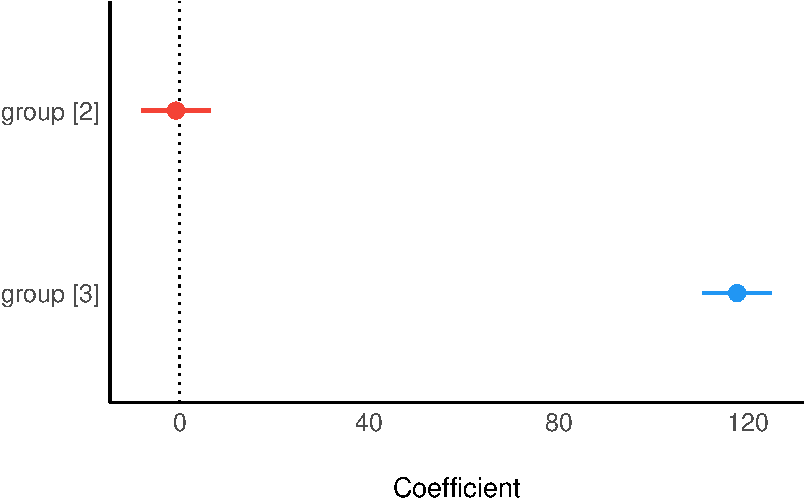
\includegraphics{02-content_files/figure-pdf/unnamed-chunk-15-1.pdf}

\subsubsection{Exercise 3}\label{exercise-3}

Perform a linear regression analysis using R. Follow the detailed
instructions below to simulate the necessary data, execute the
regression, and report your findings:

\begin{enumerate}
\def\labelenumi{\arabic{enumi}.}
\tightlist
\item
  \textbf{Simulate Data:}

  \begin{itemize}
  \tightlist
  \item
    Generate two continuous variables, \texttt{Y} and \texttt{A}, with
    \texttt{n\ =\ 100} observations each.
  \item
    The variable \texttt{A} should have a mean of \texttt{50} and a
    standard deviation (\texttt{sd}) of \texttt{10}.
  \end{itemize}
\item
  \textbf{Define the Relationship:}

  \begin{itemize}
  \tightlist
  \item
    Simulate the variable \texttt{Y} such that it is linearly related to
    \texttt{A} with a specified effect size. The effect size of
    \texttt{A} on \texttt{Y} must be explicitly defined as \texttt{2}.
  \end{itemize}
\item
  \textbf{Incorporate an Error Term:}

  \begin{itemize}
  \tightlist
  \item
    When simulating \texttt{Y}, include an error term with a standard
    deviation (\texttt{sd}) of \texttt{20} to introduce variability.
  \end{itemize}
\item
  \textbf{Regression Analysis:}

  \begin{itemize}
  \tightlist
  \item
    Use the \texttt{lm()} function in R to regress \texttt{Y} on
    \texttt{A}.
  \item
    Ensure the regression model captures the specified effect of
    \texttt{A} on \texttt{Y}.
  \end{itemize}
\item
  \textbf{Report the Results:}

  \begin{itemize}
  \tightlist
  \item
    Output the regression model summary to examine the coefficients,
    including the effect of \texttt{A} on \texttt{Y}, and assess the
    model's overall fit and significance.
  \end{itemize}
\end{enumerate}

Here is a template to get you started. Copy the code and paste it into
your R script.

\begin{Shaded}
\begin{Highlighting}[]
\FunctionTok{library}\NormalTok{(parameters)}
\CommentTok{\#  seed for reproducibility}
\FunctionTok{set.seed}\NormalTok{( ) }\CommentTok{\# numbers go in brackets}

\CommentTok{\# number of observations}
\NormalTok{n }\OtherTok{\textless{}{-}}   \CommentTok{\# number goes here}

\CommentTok{\# simulate data for variable A with specified mean and sd}
\NormalTok{A }\OtherTok{\textless{}{-}} \FunctionTok{rnorm}\NormalTok{(n, }
           \AttributeTok{mean =}\NormalTok{ , }\CommentTok{\# set your number here }
           \AttributeTok{sd =}\NormalTok{ )}\CommentTok{\# set your number here }

\CommentTok{\# define the specified effect size of A on Y}
\NormalTok{beta\_A }\OtherTok{\textless{}{-}}   \CommentTok{\# define your effect with a number here }


\CommentTok{\# simulate data and make data frame in one step}

\NormalTok{df\_3 }\OtherTok{\textless{}{-}} \FunctionTok{data.frame}\NormalTok{(}
  \CommentTok{\# simulate data for variable A with specified mean and sd}
  \AttributeTok{A =}\NormalTok{ A, }\CommentTok{\# from above}
  \AttributeTok{Y =} \DecValTok{5} \SpecialCharTok{+}\NormalTok{ beta\_A }\SpecialCharTok{*}\NormalTok{ A }\SpecialCharTok{+} \FunctionTok{rnorm}\NormalTok{(n, }\AttributeTok{mean =} \DecValTok{0}\NormalTok{, }\AttributeTok{sd =} \DecValTok{20}\NormalTok{) }\CommentTok{\#  effect is intercept + ...}
\NormalTok{)}

\CommentTok{\# view}
\FunctionTok{head}\NormalTok{(df\_3)}
\FunctionTok{str}\NormalTok{(df\_3)}

\CommentTok{\#  linear regression of Y on A}
\NormalTok{fit\_3 }\OtherTok{\textless{}{-}} \FunctionTok{lm}\NormalTok{(Y }\SpecialCharTok{\textasciitilde{}}\NormalTok{ A, }\AttributeTok{data =}\NormalTok{ df\_3)}

\CommentTok{\#  results (standard code)}
\CommentTok{\# summary(model)}

\CommentTok{\# time saving reports}
\NormalTok{parameters}\SpecialCharTok{::}\FunctionTok{model\_parameters}\NormalTok{(fit\_3)}
\FunctionTok{report}\NormalTok{(fit\_3)}
\end{Highlighting}
\end{Shaded}

\paragraph{Step 5: Simulating Data
Frames}\label{step-5-simulating-data-frames}

Data frames are used in R to store data tables. To simulate a dataset
with both continuous and categorical data, you can combine the above
steps:

\begin{Shaded}
\begin{Highlighting}[]
\CommentTok{\# create a data frame with simulated data for ID, Gender, Age, and Income}
\NormalTok{data\_frame }\OtherTok{\textless{}{-}} \FunctionTok{data.frame}\NormalTok{(}
  \CommentTok{\# generate a sequence of IDs from 1 to n}
  \AttributeTok{ID =} \DecValTok{1}\SpecialCharTok{:}\NormalTok{n,}
  
  \CommentTok{\# randomly assign \textquotesingle{}Male\textquotesingle{} or \textquotesingle{}Female\textquotesingle{} to each observation}
  \AttributeTok{Gender =} \FunctionTok{sample}\NormalTok{(}\FunctionTok{c}\NormalTok{(}\StringTok{"Male"}\NormalTok{, }\StringTok{"Female"}\NormalTok{), n, }\AttributeTok{replace =} \ConstantTok{TRUE}\NormalTok{),}
  
  \CommentTok{\# simulate \textquotesingle{}Age\textquotesingle{} data: normally distributed with mean 30 and sd 5}
  \AttributeTok{Age =} \FunctionTok{rnorm}\NormalTok{(n, }\AttributeTok{mean =} \DecValTok{30}\NormalTok{, }\AttributeTok{sd =} \DecValTok{5}\NormalTok{),}
  
  \CommentTok{\# simulate \textquotesingle{}Income\textquotesingle{} data: normally distributed with mean 50000 and sd 10000}
  \AttributeTok{Income =} \FunctionTok{rnorm}\NormalTok{(n, }\AttributeTok{mean =} \DecValTok{50000}\NormalTok{, }\AttributeTok{sd =} \DecValTok{10000}\NormalTok{)}
\NormalTok{)}
\end{Highlighting}
\end{Shaded}

Note that you can sample probabilistically for your groups

\begin{Shaded}
\begin{Highlighting}[]
\NormalTok{n }\OtherTok{\textless{}{-}} \DecValTok{100} \CommentTok{\# total number of observations}

\CommentTok{\# sample \textquotesingle{}Gender\textquotesingle{} with a 40/60 proportion for Male/Female}
\NormalTok{Gender }\OtherTok{=} \FunctionTok{sample}\NormalTok{(}\FunctionTok{c}\NormalTok{(}\StringTok{"Male"}\NormalTok{, }\StringTok{"Female"}\NormalTok{), n, }\AttributeTok{replace =} \ConstantTok{TRUE}\NormalTok{, }\AttributeTok{prob =} \FunctionTok{c}\NormalTok{(}\FloatTok{0.4}\NormalTok{, }\FloatTok{0.6}\NormalTok{))}
\end{Highlighting}
\end{Shaded}

\subsection{More complexity}\label{more-complexity}

\begin{Shaded}
\begin{Highlighting}[]
\CommentTok{\# set the number of observations}
\NormalTok{n }\OtherTok{\textless{}{-}} \DecValTok{100}

\CommentTok{\# simulate the \textquotesingle{}Age\textquotesingle{} variable}
\NormalTok{mean\_age }\OtherTok{\textless{}{-}} \DecValTok{30}
\NormalTok{sd\_age }\OtherTok{\textless{}{-}} \DecValTok{5}
\NormalTok{Age }\OtherTok{\textless{}{-}} \FunctionTok{rnorm}\NormalTok{(n, }\AttributeTok{mean =}\NormalTok{ mean\_age, }\AttributeTok{sd =}\NormalTok{ sd\_age)}

\CommentTok{\# define coefficients explicitly}
\NormalTok{intercept }\OtherTok{\textless{}{-}} \DecValTok{20000}   \CommentTok{\# Intercept for the income equation}
\NormalTok{beta\_age }\OtherTok{\textless{}{-}} \DecValTok{1500}     \CommentTok{\# Coefficient for the effect of age on income}
\NormalTok{error\_sd }\OtherTok{\textless{}{-}} \DecValTok{10000}    \CommentTok{\# Standard deviation of the error term}

\CommentTok{\# simulate \textquotesingle{}Income\textquotesingle{} based on \textquotesingle{}Age\textquotesingle{} and defined coefficients}
\NormalTok{Income }\OtherTok{\textless{}{-}}\NormalTok{ intercept }\SpecialCharTok{+}\NormalTok{ beta\_age }\SpecialCharTok{*}\NormalTok{ Age }\SpecialCharTok{+} \FunctionTok{rnorm}\NormalTok{(n, }\AttributeTok{mean =} \DecValTok{0}\NormalTok{, }\AttributeTok{sd =}\NormalTok{ error\_sd)}

\CommentTok{\# create a data frame to hold the simulated data}
\NormalTok{data\_complex }\OtherTok{\textless{}{-}} \FunctionTok{data.frame}\NormalTok{(Age, Income)}
\end{Highlighting}
\end{Shaded}

\paragraph{Step 7: Visualising Simulated
Data}\label{step-7-visualising-simulated-data}

Visualising your simulated data can help understand its distribution and
relationships. Use the \texttt{ggplot2} package for this:

\begin{Shaded}
\begin{Highlighting}[]
\FunctionTok{library}\NormalTok{(ggplot2)}
\FunctionTok{ggplot}\NormalTok{(data\_complex, }\FunctionTok{aes}\NormalTok{(}\AttributeTok{x =}\NormalTok{ Age, }\AttributeTok{y =}\NormalTok{ Income)) }\SpecialCharTok{+}
  \FunctionTok{geom\_point}\NormalTok{() }\SpecialCharTok{+}
  \FunctionTok{theme\_minimal}\NormalTok{() }\SpecialCharTok{+}
  \FunctionTok{labs}\NormalTok{(}\AttributeTok{title =} \StringTok{"Simulated Age vs. Income"}\NormalTok{, }\AttributeTok{x =} \StringTok{"Age"}\NormalTok{, }\AttributeTok{y =} \StringTok{"Income"}\NormalTok{)}
\end{Highlighting}
\end{Shaded}

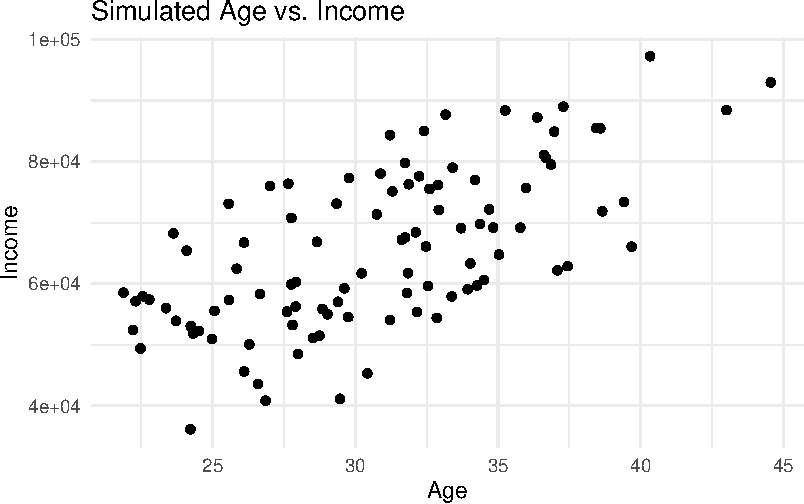
\includegraphics{02-content_files/figure-pdf/unnamed-chunk-20-1.pdf}

\subsection{Practice}\label{practice}

Simulating data is a powerful method to understand statistical concepts
and data manipulation. Let's simulate a simple dataset representing
scores from two cultural groups.

\begin{itemize}
\tightlist
\item
  \textbf{Data simulation:}
\end{itemize}

You've learned to simulate datasets in R. This is a foundational skill
for exploring statistical concepts and data manipulation techniques.
Congratulations!

\subsection{Appendix A: Solutions}\label{appendix-a}

\subsubsection{Solution Problem Set 3: simulate data and regression
reporting}\label{solution-problem-set-3-simulate-data-and-regression-reporting}

\begin{Shaded}
\begin{Highlighting}[]
\FunctionTok{library}\NormalTok{(parameters)}
\CommentTok{\#  seed for reproducibility}
\FunctionTok{set.seed}\NormalTok{(}\DecValTok{12345}\NormalTok{)}

\CommentTok{\# number of observations}
\NormalTok{n }\OtherTok{\textless{}{-}} \DecValTok{100}

\CommentTok{\# simulate data for variable A with specified mean and sd}
\NormalTok{A }\OtherTok{\textless{}{-}} \FunctionTok{rnorm}\NormalTok{(n, }\AttributeTok{mean =} \DecValTok{50}\NormalTok{, }\AttributeTok{sd =} \DecValTok{10}\NormalTok{)}

\CommentTok{\# define the specified effect size of A on Y}
\NormalTok{beta\_A }\OtherTok{\textless{}{-}} \DecValTok{2}


\CommentTok{\# simulate data and make data frame in one step}

\NormalTok{df\_3 }\OtherTok{\textless{}{-}} \FunctionTok{data.frame}\NormalTok{(}
  \CommentTok{\# simulate data for variable A with specified mean and sd}
  \AttributeTok{A =}  \FunctionTok{rnorm}\NormalTok{(n, }\AttributeTok{mean =} \DecValTok{50}\NormalTok{, }\AttributeTok{sd =} \DecValTok{10}\NormalTok{),}
  \AttributeTok{Y =} \DecValTok{5} \SpecialCharTok{+}\NormalTok{ beta\_A }\SpecialCharTok{*}\NormalTok{ A }\SpecialCharTok{+} \FunctionTok{rnorm}\NormalTok{(n, }\AttributeTok{mean =} \DecValTok{0}\NormalTok{, }\AttributeTok{sd =} \DecValTok{20}\NormalTok{)}
\NormalTok{)}

\CommentTok{\# view}
\FunctionTok{head}\NormalTok{(df\_3)}
\end{Highlighting}
\end{Shaded}

\begin{verbatim}
         A         Y
1 52.23925  87.98766
2 38.43777 106.60413
3 54.22419 107.68437
4 36.75245 117.09730
5 51.41084 133.74473
6 44.63952  70.74512
\end{verbatim}

\begin{Shaded}
\begin{Highlighting}[]
\FunctionTok{str}\NormalTok{(df\_3)}
\end{Highlighting}
\end{Shaded}

\begin{verbatim}
'data.frame':   100 obs. of  2 variables:
 $ A: num  52.2 38.4 54.2 36.8 51.4 ...
 $ Y: num  88 107 108 117 134 ...
\end{verbatim}

\begin{Shaded}
\begin{Highlighting}[]
\CommentTok{\# Perform linear regression of Y on A}

\NormalTok{fit\_3 }\OtherTok{\textless{}{-}} \FunctionTok{lm}\NormalTok{(Y }\SpecialCharTok{\textasciitilde{}}\NormalTok{ A, }\AttributeTok{data =}\NormalTok{ df\_3)}

\CommentTok{\# Report the results of the regression}
\CommentTok{\# summary(model)}

\CommentTok{\# report}
\NormalTok{parameters}\SpecialCharTok{::}\FunctionTok{model\_parameters}\NormalTok{(fit\_3)}
\end{Highlighting}
\end{Shaded}

\begin{verbatim}
Parameter   | Coefficient |    SE |          95% CI | t(98) |      p
--------------------------------------------------------------------
(Intercept) |      109.17 | 14.62 | [80.17, 138.18] |  7.47 | < .001
A           |   -3.80e-03 |  0.28 | [-0.57,   0.56] | -0.01 | 0.989 
\end{verbatim}

\begin{Shaded}
\begin{Highlighting}[]
\FunctionTok{report}\NormalTok{(fit\_3)}
\end{Highlighting}
\end{Shaded}

\begin{verbatim}
We fitted a linear model (estimated using OLS) to predict Y with A (formula: Y
~ A). The model explains a statistically not significant and very weak
proportion of variance (R2 = 1.83e-06, F(1, 98) = 1.79e-04, p = 0.989, adj. R2
= -0.01). The model's intercept, corresponding to A = 0, is at 109.17 (95% CI
[80.17, 138.18], t(98) = 7.47, p < .001). Within this model:

  - The effect of A is statistically non-significant and negative (beta =
-3.80e-03, 95% CI [-0.57, 0.56], t(98) = -0.01, p = 0.989; Std. beta =
-1.35e-03, 95% CI [-0.20, 0.20])

Standardized parameters were obtained by fitting the model on a standardized
version of the dataset. 95% Confidence Intervals (CIs) and p-values were
computed using a Wald t-distribution approximation.
\end{verbatim}

\subsection{What You Have Learned}\label{what-you-have-learned}

\begin{itemize}
\tightlist
\item
  \textbf{Data simulation:}
\end{itemize}

You've learned to simulate datasets in R. This is a foundational skill
for exploring statistical concepts and data manipulation techniques.
Congratulations!

\begin{itemize}
\tightlist
\item
  \textbf{Data visualisation:}
\end{itemize}

You've begun data visualising data through boxplots and histograms and
coefficient plots, which is crucial for analysing and communicating
statistical findings.

\begin{itemize}
\item
  \textbf{Statistical tests:} You've conducted basic statistical tests,
  including t-tests and ANOVA, gaining insights into comparing means
  across groups.
\item
  \textbf{Understanding ANOVA and regression:}
\end{itemize}

You've explored the equivalence of ANOVA and regression analysis,
learning how these methods can be applied to analyse and interpret data
effectively.

\subsection{For more information about the packages used
here:}\label{for-more-information-about-the-packages-used-here}

\begin{itemize}
\item
  \href{https://ggplot2.tidyverse.org/}{ggplot2}: A system for
  declaratively creating graphics, based on The Grammar of Graphics.
\item
  \href{https://easystats.github.io/parameters/}{Parameters package}:
  Provides utilities for processing model parameters and their metrics.
\item
  \href{https://easystats.github.io/report/index.html}{Report package}:
  Facilitates the automated generation of reports from statistical
  models.
\end{itemize}

\subsection{Appendix A: I lied}\label{appendix-a-i-lied}

We can get group comparisons with ANOVA, for example:

\begin{Shaded}
\begin{Highlighting}[]
\CommentTok{\# Conduct Tukey\textquotesingle{}s HSD test for post{-}hoc comparisons}
\NormalTok{tukey\_post\_hoc }\OtherTok{\textless{}{-}} \FunctionTok{TukeyHSD}\NormalTok{(anova\_model)}

\CommentTok{\# Display the results}
\FunctionTok{print}\NormalTok{(tukey\_post\_hoc)}
\end{Highlighting}
\end{Shaded}

\begin{verbatim}
  Tukey multiple comparisons of means
    95% family-wise confidence level

Fit: aov(formula = y ~ group, data = df_1)

$group
           diff        lwr        upr     p adj
2-1  -0.8030143  -9.560281   7.954253 0.9739971
3-1 117.6732276 108.915961 126.430495 0.0000000
3-2 118.4762419 109.718975 127.233509 0.0000000
\end{verbatim}

\begin{Shaded}
\begin{Highlighting}[]
\FunctionTok{plot}\NormalTok{(tukey\_post\_hoc)}
\end{Highlighting}
\end{Shaded}

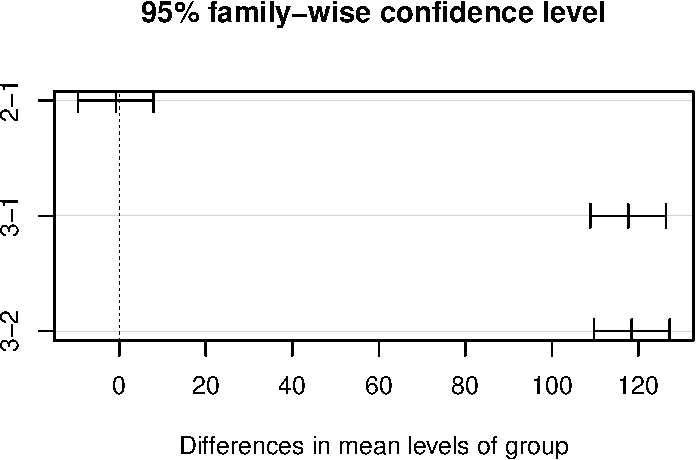
\includegraphics{02-content_files/figure-pdf/unnamed-chunk-22-1.pdf}

Regression and ANOVA are equivalent



\end{document}
